%
% File coling2020.tex
%
% Contact: feiliu@cs.ucf.edu & liang.huang.sh@gmail.com
%% Based on the style files for COLING-2018, which were, in turn,
%% Based on the style files for COLING-2016, which were, in turn,
%% Based on the style files for COLING-2014, which were, in turn,
%% Based on the style files for ACL-2014, which were, in turn,
%% Based on the style files for ACL-2013, which were, in turn,
%% Based on the style files for ACL-2012, which were, in turn,
%% based on the style files for ACL-2011, which were, in turn, 
%% based on the style files for ACL-2010, which were, in turn, 
%% based on the style files for ACL-IJCNLP-2009, which were, in turn,
%% based on the style files for EACL-2009 and IJCNLP-2008...

%% Based on the style files for EACL 2006 by 
%%e.agirre@ehu.es or Sergi.Balari@uab.es
%% and that of ACL 08 by Joakim Nivre and Noah Smith

\documentclass[11pt]{article}
\usepackage{coling2020}
\usepackage{times}
\usepackage{amsmath,amsfonts,amssymb}
\usepackage{url}
\usepackage{latexsym}
\usepackage{hyperref}
\usepackage[noabbrev,capitalize]{cleveref}
\usepackage{graphicx}
\usepackage{subcaption}
\usepackage{pgfplots}
\usepackage{wrapfig}
\pgfplotsset{every tick label/.append style={font=\small}}

\newcommand\jp[1]{(\textbf{JP:} #1)}
\newcommand\adam[1]{(\textbf{Adam:} #1)}
\newcommand\citet{\newcite}
\newcommand\citep{\cite}
\newcommand\citeyear{\shortcite}
\newcommand\softmax{\mathsf{softmax}}
%\setlength\titlebox{5cm}
%\colingfinalcopy % Uncomment this line for the final submission

% You can expand the titlebox if you need extra space
% to show all the authors. Please do not make the titlebox
% smaller than 5cm (the original size); we will check this
% in the camera-ready version and ask you to change it back.


\title{Composing Byte-Pair Encodings for Morphological Sequence Classification}


\author{Adam Ek \and Jean-Philippe Bernardy\\
	Centre for Linguistic Theory and Studies in Probability,\\
	Department of Philosophy, Linguistics and Theory of Science,\\
	University of Gothenburg,\\
	\texttt{\{adam.ek, jean-philippe.bernardy\}@gu.se}}

\date{}

\begin{document}
	\maketitle
	
	\begin{abstract}
		\jp{TODO}. This document contains the instructions for preparing a paper submitted
		to COLING-2020 or accepted for publication in its proceedings. The document itself
		conforms to its own specifications, and is therefore an example of
		what your manuscript should look like. These instructions should be
		used for both papers submitted for review and for final versions of
		accepted papers. Authors are asked to conform to all the directions
		reported in this document.
	\end{abstract}
	
	\section{Introduction}
	\label{intro}

            After its introduction [CITE:TODO], the transformer model
     \citep{vaswani2017attention} has emerged as the dominant
     architecture for statistical language models, displacing
     recurrent neural networks, in particular the LSTM and its
     variants. The transformer owes its success to several factors,
     including the availability of pretrained models, which
     effectively yield rich contextual word embeddings. Such
     embeddings can be used as is (for so-called \emph{feature extraction}),
     or the pre-trained models can be fine-tuned to specific
     applications.

    	At the same time as transformer models became popular, the
     tokenization of natural language texts have shifted away from
     methods explicitly oriented on words or morphemes. Rather,
     statistical approaches are favoured: strings of
     characters are split into units which are not necessarily meaningful
     linguistically, but rather have statistically balanced
     frequencies. For example, the word "scientifically" may be
     composed of the tokens: "scient", "ifical", "ly" --- here the
     central token does not correspond to a morpheme.
        %
         That is, rather than identifying complete words or morphemes,
     one aims to find relatively large sub-word units occurring
     significantly often, while maximizing the coverage of the corpus
     (the presence of the ``out of vocabulary'' token is
     minimized). Approaches for composing tokens from sub-token
     units have focused on combining character $n$-grams
     \citep{bojanowski2017enriching}, while other approaches have
     looked at splitting words into \textit{roots} and
     \textit{morphemes}
     \citep{el2012orthographic,chaudhary2018adapting,xu2017implicitly},
     and then combining them. In this paper, we consider in particular
     Byte-Pair Encodings (BPE) \citep{sennrich2015neural}, which takes
     another approach. It does not specifically look for either
     character $n$-grams or morphs, but rather it aims at splitting a
     corpus $\mathcal{C}$ into $N$ tokens, where $N$ is user
     defined.

                One issue with statistical tokenization, such as BPE,
     is that one is seldom interested in the encoding, but rather in
     the semantically meaningful units in the original texts. Thus the
     question of mapping results back to the original text arises.

        	In this paper we explore how to combine Byte-Pair
     Encodings from a transformer model to perform sequence
     classification, which is used in the popular BERT model
     \citep{devlin2018bert}. For our purposes, the goal in sequence
     classification is to assign a label to every word in a
     sentence. When we are using byte-pair encoding (or similar
     sub-token representations) we must then find some way of
     combining the units that compose the word, before it is
     eventually assigned a label. Coming back to our example, we must
     map the feature-set assigned (depending on the context) to
     "scient", "ifical" and "ly". Then this combined feature set is
     mapped to a class for the whole word ``scientifically''.

    %\begin{table}  
    %\centering  
    %\begin{tabular}{lllll}
    %Wordform & \multicolumn{4}{l}{teyzelerin} \\
    %Segmentation & teyze & ler in \\
    %BPE segmentation & te & y & ze & lerin \\
    %\end{tabular}
    %\caption{Turkish example}
    %\label{tab:t_example}
    %\end{table}

                	To our knownledge, this is a little-studied
     problem. For the original BERT model \citet{devlin2018bert} simply
     state that for named entity recognition the first sub-word token
     is used as a representation for the word to be tagged.  For
     morphological sequence classification \citet{kondratyuk2019cross}
     report that only few differences were found between averaging,
     taking the first or last sub-word token feature set.  In this paper we wish
     to explore the problem in further detail and identify the effect
     that different methods have on the final performance of a model.

     Even though BPE is not grounded in morphosyntactic theory, the
     characteristics of the BPE embeddings will be directly influenced
     by morphosyntactic patterns in the language. In particular, it is
     reasonable to expect that the statistical characteristics of BPE
     to be different between fusional and agglutinative languages.
     %
     Additionally, with the increased interest in multilingual NLP it
     becomes important to explore how ``universal'' different
     computational methods are.  That is, because languages are
     different (morpho-)syntactically, % {orthographically and grammatically}
     one can expect the
     methods to derive information not to be uniformly
     efficient.

     However, at the same time, researchers always strive
     to find unified theories and models, working for all language
     families.
     %
     In statistical models, one tends to unify models by adding more
     parameters to them, and then feeding them with correspondingly
     more data.  In theory, more data is often possible to find,
     because languages are infinite, and exhibit a large variance in
     their usage. But this variability is also a source of confusion
     for the statistical models. Hence, in sum, one should always be
     on the lookout for the most efficient \emph{method} to model
     languages and solve tasks. This is our aim: finding the best
     methods for BPE combination, by analysing them in various
     contexts.

    \section{Task}
             In this paper we focus on the task of
     morphological sequence classification. Morphological tagging
     involves identifying a set of morphological features that a word
     possesses, such as number, person, case, etc. In many languages,
     morphological features primarily depend on the affixes of
     words. However, conversely, the morphological class is not
     determined by the word affixes, nor even the whole word. In many
     cases, the context of the sentence will affect which class should
     be assigned to a word.

     For our task, we have to identify $k$ different tags for a word,
     each with $C_i$ possible classes, making the task a multi-class
     classification problem. We simplify the classification problem by
     combining the different tags into a composite tag with up to
     $\prod _i^k C_i$ classes (instead of making $k$ separate
     predictions).

    \section{Data}
    
    For both training and testing data, we use the Universal
    Dependencies dataset \citep{nivre2018} annotated with the UniMorph
    schema \citep{mccarthy2018marrying}. We are interested in how
    accuracy is influenced by different composition methods, and by
    the typology of the languages. Additionally, we also consider the
    correlation between these two variables --- still in terms of the
    effect on accuracy for the task. To this end, we take a sample
    of eight languages from the Universal Dependencies dataset. Four
    languages use a \textit{fusional} morphology, meaning that an
    affix may be indicative of one or more morphological features. The
    other four languages use an \textit{agglutinative} morphology,
    meaning that each affix is mapped to one and only one
    morphological feature.

           	The fusional languages that we consider are Arabic, Czech,
     Polish and Spanish, and the agglutinative languages that we
     consider are Finnish, Basque, Turkish and Estonian.  We show the
     size, average number of BPE tokens per text-token and number of
     morphological tags for each treebank in \cref{tab:data}.
    
    %The size of
    % the dataset \jp{in original words?}  and the average number of
    % BPE tokens per word are shown in \cref{tab:data}.

    
    
    	\begin{table} % JP it's better to leave placement to the tex engine and the style sheet. (unless there is a real problem doing so)
		\centering
		\begin{tabular}{l|lrrrrr}
			Language & Typology & $\frac{BPE}{word}$ & Tags & Train & Validation & Test \\
			\hline
			Basque-BDT      & Agglutinative & 1.79 & 919 & 97336 & 12206 & 11901 \\
			Finnish-TDT     & Agglutinative & 1.98 & 591 & 161791 & 19876 & 20541 \\
			Turkish-IMST    & Agglutinative & 1.73 & 1056 & 46417 & 5708 & 5734 \\
			Estonian-EDT    & Agglutinative & 1.86 & 512 & 346986 & 43434 & 43825 \\
            Arabic-PADT     & Fusional & 1.39 & 300 & 225494 & 28089 & 28801  \\
			Czech-CAC       & Fusional & 1.77 & 990 & 395043 & 50087 & 49253 \\
			Polish-LFG      & Fusional & 1.75 & 634 & 104730 & 13161 & 13076 \\
			Spanish-AnCora  & Fusional & 1.25 & 177 & 439925 & 55196 & 54449 \\
        \end{tabular}
    		\caption{\label{tab:data} Treebank statistics showing the
     language typology, average number of BPE tokens per word, the
     number of morphological tags and the size of the datasets in
     terms of text tokens.}
	\end{table}
    
        The fusional languages where chosen such that two of them
        (Czech and Polish) have a higher BPE per token ratio than the
        other two (Arabic and Spanish). We make this choice because
        one factor that impacts the accuracy obtained by a composition
        method may be the BPE per token ratio.  By having both
        fusional and agglutinative languages with similar BPE per
        token ratio we can take this variable into account properly in
        our analysis.
    % \jp{But we never come back to this point? AE: as of yet, the current experiments do not seem to yield same results as before}
        \jp{So what is the status? forward ref to the precise point where this is discussed?}
        
	\section{Method}
	\label{method}
    	In this section we present the model used for sequence
     classification, the methods that we use to compose BPE
     embeddings, and how we trained the model. \footnote{Our code is
     available at: \url{https://github.com/ANONYMIZED}}

	\subsection{Model}

        Our model is composed of three components, each of them
        detailed below. First, the input sequence of BPE tokens is fed
        to a transformer model, which yields a feature set for each
        BPE token. Then, the BPE tokens are combined using a
        composition module, which we vary for the purpose of
        evaluating each variant. This component yield one feature set
        per original word. Then a bidirectional LSTM is applied, which
        is followed by two dense layers with GELU\jp{Gaussian Error Linear Units? If so cite: https://arxiv.org/abs/1606.08415}
        activation. These dense layers act on each word separately (but
        share parameters accross words).  An outline of the model is
        presented in \cref{fig:model}, where $f$ represents the
        different methods we use to combine BPE embeddings.

	\subsubsection{Underlying Transformer Model}
     To extract a feature set for BPE tokens, we use the
     XLM-RoBERTa \cite{conneau2019unsupervised} model\footnote{We use the
     huggingface implementation
     \url{https://huggingface.co/transformers/model_doc/xlmroberta.html}}. XLMR
     is a masked language model based on the transformer
     (specifically RoBERTa \citep{liu2019roberta}), and trained on
     data from 100 different languages, using a shared vocabulary of
     250000 BPE tokens. All the languages that we test are included in the
     XLMR model. In this experiment we use the \textsc{XLMR}$_{base}$
     model. It has 12 encoder layers, 12 attention heads and use 768
     dimensions for its hidden size.

	\subsubsection{BPE feature extraction}
        \label{sec:bpe-features}

        % As mentioned previously, we look at methods for composing embeddings of BPE tokens into word embeddings.

                The XLMR model use 12 layers to compute an embedding
     for a BPE token, and it has been shown in previous research
     \citep{kondratyukstraka,raganato2018analysis,liu2019linguistic}
     \adam{[Find 1 or 2 more citations]} that the different layers of the
     transformer model encode different types of information. To take
     advantage of this variety, we compute BPE embeddings as a weighted sum of
     layer representations \citep{kondratyukstraka}.  That is, we
     initialize a parameter $w$ of dimension $l$, each element from a normal
     distribution of mean $0$ and standard deviation $1$, where $l$ is
     the number of layers in the transformer model. If $r_{ji}$ is the
     layer representation at layer $j$ and token position $i$, we
     calculate the weighted sum as follows:
    \begin{equation}
		x_i = \sum_{j=1}^{l} \softmax(w)_j r_{ji}
	\end{equation}

        Consequently, in end-to-end training, the optimiser will find
        a weight for extracting information from each layer
        ($\softmax(w)_j$) which maximizes performance.

     \subsubsection{Composition of BPE feature sets}
      After we have computed a weighted sum for
     each BPE token we proceed to combine them into the tokens as they
     appear in the data.
	The model that we use to combine morphological features is as
        follows. For each sentence we extract $n$ BPE embeddings $x^0$
        to $x^{n-1}$ from $XLMR_{base}$, and then align them to
        words.

        We then feed all words which consist of more than one
        BPE embedding to a function $f$ which combines the BPE
        embeddings.

        We consider three methods: summation,
        averaging, and using an RNN. Summation and
        averaging have been used in previous work \adam{[CITATIONS]}, but
        using an RNN have not been explored before to our knowledge.
    
    	\paragraph{Sum:} For the sum method, we use an element-wise
     sum. That is, we take the sum for each dimension of the BPE
     embeddings independently. Thus, for token $i$ we calculate a
     composite embedding by summing over dimensions $1,\ldots,D$:
	
	\begin{equation}
	f(x)_i = \sum_{j=1}^{D} x_i^j
	\end{equation}
	

    	\paragraph{Mean:} In the mean method we calculate the sum as above and
     divide by the number of BPE embeddings in the word. Thus, for
     token $i$ we calculate a composite embedding by averaging over
     dimensions $1,\ldots,D$:
	
	\begin{equation}
	f(x)_{i} = \frac{1}{D}\sum_{j=1}^{D} x_i^j
	\end{equation}
	
	
        	\paragraph{RNN:} For this method we employ a bidirectional
     LSTM to compose the BPE embeddings. For each multi-BPE token, we
     pass the sequence of BPE embeddings through an LSTM and use the
     final output as our word representation.

        \subsubsection{Word-level feature sets and classification}
        The above produces one embedding per word that is passed to an
        LSTM (regardless of the method), to take into account the
        context.

        \jp{Is using character features a common technique? If so say it, if not not then the next sentence should be deleted.}
        We opted not to include character
        features because these would obfuscate the effect of the composition
        method and may mask some of the effects of the different
        methods.

        We pass the combined representations to LSTM outputs to a
        dense layers with GELU activation, that computes scores
        for each class in the output. We then use a softmax layer to
        assign probabilities, and compute the loss accordingly.

	\begin{figure}%[h!]
          \centering
	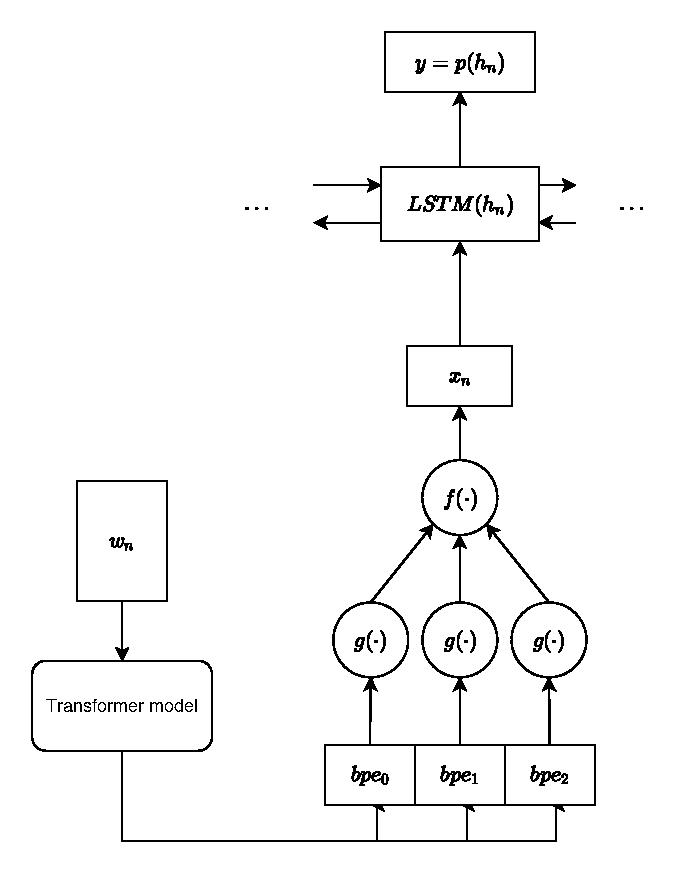
\includegraphics[scale=0.5]{single_step.pdf}
    \caption{\label{fig:model} Model outline for one input. A
     word $w_n$ is tokenized into $k$ BPE tokens by the transformer
     model, we then calculate a weighted sum over the layers for each
     feature embedding in a function $g(\cdot)$ \jp{What is this g? Why isn't it explained before? Perhaps it could be deleted from here?}. The resulting
     embeddings are then passed to a BPE composition function
     $f(\cdot)$ that combines the $k$ different BPE embeddings into a
     word embedding. The word embedding is then passed to a LSTM
     followed by a dense preiction layer. }
	\end{figure}

	%\subsubsection{Character features}
    %    \jp{Delete? Keep?}
    %	In addition to layer attention we use a character LSTM to
    % extract a word representation based on characters. The final
    % representation that we pass to the word-LSTM is the concatenation
    % of the word representation based on BPE compositions and
    % characters,
    % $w_i = \text{concat}(f(bpe_0,...,bpe_K), f(c_0, ..., c_M))$
	
	\subsubsection{Label smoothing}
    	Given that many of the languages have a large number of
     morphological tags, we want to prevent the model from growing
     overconfident for certain classes. To address this issue we
     introduce label smoothing \cite{szegedy2016rethinking}, that is,
     instead of the incorrect classes having $0\%$ probability and the
     correct class $100\%$ probability we let each of the incorrect
     classes have a small probability.

        %The correct class is then assigned the probability $t$ by
     %$(1-\alpha)t + \alpha / |C|$ where $|C|$ is the number of
     %classes. \jp{I don't understand this formula (and I botched the
     %sentence trying to fix it :/ ... What is $t$? I was expecting
     %that you'd give the formula for the probability of the correct
     %class, but apparently I am mistaken.)}

     Let $\alpha$ be our smoothing value \jp{What is the value of
       alpha used?}  and $C$ the number of classes, then given a
     one-hot encoded target vector $t$ of size $C$, we calculate the
     smoothed probabilities as:
    \begin{equation}
        t_{smooth} = (1-\alpha)t + \frac{\alpha}{C}
    \end{equation}
    In words, we remove $\alpha$ from the correct class then
    distribute $\alpha$ uniformly among all classes.
     \subsection{Training}

    %\jp{add here a warning that we consider several possible training regimes}
	
     In our experiments we consider two possible training regimes. In
     the first regime we finetune the XLMR models parameters, in the
     second regime we only extract weights for BPE tokens, that is, we
     use the model as a feature extractor. In all cases, we use
     end-to-end training.

    	\begin{wraptable}{r}{5cm}
		\centering
		\begin{tabular}{lr} \\
			Parameter & Value \\
			\hline
			Epochs & 15 \\
			Batch size & 4 / 32 \\
			%Character representation size & 128 \\
            Word LSTM size & 768 \\
            Linear transform size & 1536 \\
			% optimizers
			Optimizer & Adam \\
			Learning rate & 0.001 \\
			Learning rate$_{xlmr}$ & 1e-06 \\
			% regularization
            Weight decay & 0.05 \\
			Label smoothing & 0.03 \\
            % described in text
            %Prediction dropout & 0.5 \\
			%Transformer dropout & 0.4 \\
            %Layer dropout & 0.1 \\
            %Input dropour & 0.2 \\
            %BPE dropout & 0.4 \\
            %Character dropout & 0.4 \\
		\end{tabular}
    		\caption{\label{tab:parameters} Hyperparameters used for
     training the model. Slashed indicate the value of a parameter
     when we finetune or extract features.}
	\end{wraptable}
     
         When fine-tuning the model we freeze the XLMR parameters for
     the first epoch, (effectively not fine-tuning at first).  When training the model we use a cosine annealing learning
     rate with restarts every epoch, that is, the learning rate starts
     high then incrementally decreases to $1\mathrm{e}{-12}$ during
     $N$ steps, where $N$ is the number of batches in an epoch. We use
     the Adam optimizer, using standard parameters, with a learning
     rate of $0.001$ for layer importance parameter ($w$ in
     \cref{sec:bpe-features}), the parameters of the word LSTM,
     classification layer, and BPE combination module (when an RNN is
     used). For the transformer parameters, we use a lower learning
     rate of $1\mathrm{e}{-06}$. We summarize the hyperparameters used
     in \cref{tab:parameters}.



        We use dropout throughout the model. We apply dropout on the
        input to the transformer, replacing 20 percent of the BPE tokens
        with \texttt{<UNK>}. After we have extracted layer features
        from the transformer we apply a dropout of $0.4$, and before
        computing the weighted sum of layers we apply full\jp{What is full dropout (compared to just dropout?)} dropout on
        a layers with a probability of $0.1$. After the word LSTM have
        processed the sequence, but before the final prediction, we
        apply a dropout of $0.5$.

	
	\section{Results}
	\label{results}

         Even though our aim is to compare the relative performance of
     various BPE combination methods rather than to improve on the
     state of the art in absolute terms, we compare our results
     against the baseline reported by
     \citet{mccarthy2019sigmorphon}. This comparison serves the
     purpose of checking that our system is generally sound.  In
     particular, the actual state of the art, as reported by
     \citet{mccarthy2019sigmorphon,kondratyuk2019cross}, use treebank
     concatenation or other methods to incorporate information from
     all treebanks available in a language, which means that results
     are not reported on a strict per-treebank basis --- contrary to
     what we do here --- and thus our numbers are not directly comparable.
        % get new ref from shared task to kondratyukstraka, and perhaps other systems
    %
        The accuracy of our system is computed by checking the prediction
        of morphological tags. We report in \cref{tab:results_tokens}
        the result for each of the three different methods, and the
        two training regimes.

%	\begin{table} % [h]
%	%\small
%	\centering
%	\begin{tabular}{l|c|ccc|ccc}
%		& & \multicolumn{3}{c}{Finetuning} & \multicolumn{3}{c}{Feature extraction} \\
%		Treebank & Baseline & Sum & Mean & RNN & Sum & Mean & RNN \\
%		\hline
%		% agglutinative languages
%        Basque-BDT      & .676 & .905 & .906 & \textbf{.920} & .865 & .865 & \textbf{.888} \\
%		Finnish-TDT     & .751 & .965 & .963 & \textbf{.967} & .930 & .931 & \textbf{.942} \\ 
%		Turkish-IMST    & .620 & .898 & .891 & \textbf{.905} & .856 & .849 & \textbf{.866}\\
%		Estonian-EDT    & .740 & .960 & .961 & \textbf{.962} & .931 & .934 & \textbf{.939} \\
%		% fusional languages
%		Spanish-AnCora  & .842 & .979 & .979 & \textbf{.980} & .968 & .967 & \textbf{.971} \\
%		Arabic-PADT     & .770 & .952 & .953 & \textbf{.954} & .941 & .939 & \textbf{.948} \\
%		Czech-CAC       & .771 & .976 & .976 & \textbf{.977} & .944 & .944 & \textbf{.952} \\
%		Polish-LFG      & .657 & .959 & .956 & \textbf{.960} & .907 & .907 & \textbf{.928} \\
%        \hline
%        Average         & .728 & .949 & .948 & \textbf{.953} & .918 & .917 & \textbf{.929} \\
%	\end{tabular}
%    	\caption{\label{tab:results_tokens} Accuracy for morphological
%        tagging. We evaluate both when we finetune the XLMR model and
%        when we only extract BPE embeddings.}
%	\end{table}

    \begin{table}%[h]
	%\small
	\centering
	\begin{tabular}{l|c|ccc|ccc}
		& & \multicolumn{3}{c}{Finetuning} & \multicolumn{3}{c}{Feature extraction} \\
		Treebank & Baseline & Sum & Mean & RNN & Sum & Mean & RNN \\
		\hline
		Basque-BDT      & .676 & .884 & .877 & \textbf{.901} & .789 & .780 & \textbf{.834} \\
		Finnish-TDT     & .751 & .958 & .960 & \textbf{.965} & .856 & .847 & \textbf{.899} \\
		Turkish-IMST    & .620 & .859 & .855 & \textbf{.884} & .741 & .735 & \textbf{.775} \\
		Estonian-EDT    & .740 & .955 & .955 & \textbf{.961} & .856 & .853 & \textbf{.901} \\
		Spanish-AnCora  & .842 & .977 & .977 & \textbf{.979} & .954 & .952 & \textbf{.962} \\
		Arabic-PADT     & .770 & .946 & .947 & \textbf{.951} & .923 & .920 & \textbf{.936} \\
		Czech-CAC       & .771 & .968 & .968 & \textbf{.975} & .887 & .881 & \textbf{.924} \\
		Polish-LFG      & .657 & .953 & .953 & \textbf{.959} & .844 & .840 & \textbf{.878} \\
        \hline
        Average         & .728 & .937 & .936 & \textbf{.946}  & .856 & .851 & \textbf{.888} \\
	\end{tabular}
    	\caption{\label{tab:results_tokens} Accuracy for morphological
        tagging. We evaluate both when we finetune the XLMR model and
        when we only extract BPE embeddings.}
    \end{table}


        Our system performs better than the baseline. As a general
        trend we see that the RNN method tends to perform better
        than the summation or averaging methods. This is consistent
        across both languages families (agglutinative and fusional),
        and training regimes, showing that while the advantage of the RNN is
        small, it occurs consistenty.\jp{Can we rule out the possibility that this is simply due to additional non-recurrent layers? One could say that the two additional dense layers already do this job and so the non-recurrent aspect is already taken care of by these last two layers(?)}
    %
        We find that in general finetuning yields higher accuracy than
        plain feature extraction, on average the difference is about $5.8$
        percentage points.  This difference is to be expected when the
        finetuning have 250M more parameters tuned to the task than the
        feature extraction. % less than expected...
    
    %which is understandable given that more
    %    parameters are tuned to the task.
    %However, the difference is
    %    negligible \jp{to say so requires statistical analysis in such
    %      a paper}, increasing by $3.1$ percentage points for
    %    summation and averaging and $2.4$ points for RNN.

        When finetuning we see the largest changes for Basque with an
        increased performance of $3.25$ points, and Turkish ($2.7$
        points) using RNN over using mean or averaging. When only
        extracting features we see a larger increase when using an
        RNN, of $3.7$ points (Turkish) and $4.95$ points
        (Basque). Again, this is not unexpected: when fine-tuning the
        smaller error rate is overall smaller and therefore there is a
        smaller margin for a subsequent phase to yield an improvement.

    \Cref{tab:results_tokens} reports average accuracy for every word,
    thus also including those which are only composed of a single BPE
    token. To highlight the strengths and weaknesses of each
    composition method, we also compute the accuracy for longer words only 
    (composed of two BPE tokens or more). The results can be seen in
    \cref{tab:results_large_tokens}.  We see again that the RNN works
    better than summation or averaging BPE embeddings.
    
	\begin{table}%[h]
	%\small
	\centering
	\begin{tabular}{l|ccc|ccc}
		 & \multicolumn{3}{c}{Finetune} & \multicolumn{3}{c}{Feature extraction} \\
		Treebank & Sum & Mean & RNN & Sum & Mean & RNN  \\
		 \hline
		% agglutinative languages
        Basque-BDT      & .802 & .790 & \textbf{.835} & .715 & .703 & \textbf{.774} \\
		Finnish-TDT     & .946 & .946 & \textbf{.952} & .805 & .794 & \textbf{.861} \\ 
		Turkish-IMST    & .780 & .778 & \textbf{.818} & .683 & .664 & \textbf{.711} \\
		Estonian-EDT    & .939 & .939 & \textbf{.949} & .805 & .803 & \textbf{.868} \\
		% fusional languages
		Spanish-AnCora  & .961 & .959 & \textbf{.964} & .937 & .930 & \textbf{.947} \\
		Arabic-PADT     & .896 & .898 & \textbf{.907} & .909 & .906 & \textbf{.923}\\
		Czech-CAC       & .947 & .947 & \textbf{.959} & .849 & .840 & \textbf{.900} \\
		Polish-LFG      & .920 & .918 & \textbf{.927} & .761 & .752 & \textbf{.812} \\
        \hline
        Average         & .899 & .897 & \textbf{.913} & .808 & .799 & \textbf{.849} \\
	\end{tabular}
    \caption{\label{tab:results_large_tokens} Accuracy for
     morphological tagging on all tokens that are composed of 2 or
     more BPE tokens.}
\end{table}

            We see the same trend for accuracy on tokens that are
     composed of two or more BPE tokens, as in the overall accuracy,
     where the RNN outperform both the sum and averaging methods. We
     can also see that the average increase in accuracy when using an
     RNN is larger. This holds for both when we only finetune the
     model and extract features.

    
    Given that the number of BPE tokens per natural-language token
     varies, we also look at the accuracy of the different methods
     given a different number of BPE tokens. We show per-language
     performance with the different methods in \cref{fig:bpe_lens}.
    
	\begin{figure}%[h!]
  	\centering\begin{tikzpicture} 
	\begin{axis}[
	name=,
	title={Finnish-TDT},
        xtick style={draw=none},
        ytick style={draw=none},
        xtick={1,2,3,3,4,5,6,7},
	typeset ticklabels with strut,
	legend pos=south west,
	ymajorgrids=false,
	grid style=dashed,
	height=4cm
	]
		\addplot[
		color=green,
		mark=circle*,
                mark size=1,
                error bars/.cd, y dir=both, y explicit,
		]
		coordinates {
			(1, 0.969671597)
			(2, 0.94797361)
			(3, 0.945349627)
			(4, 0.926686217)
			(5, 0.959302326)
			(6, 0.972222222)
			(7, 0.95)
};
		\addplot[
		color=blue,
		mark=triangle*,
                mark size=1,
                error bars/.cd, y dir=both, y explicit,
		]
		coordinates {
			(1, 0.972648618)
			(2, 0.950801131)
			(3, 0.94263408)
			(4, 0.926686217)
			(5, 0.968023256)
			(6, 0.953703704)
			(7, 0.95)
};
		\addplot[
		color=red,
		mark=square*,
                mark size=1,
                error bars/.cd, y dir=both, y explicit,
		]
		coordinates {
			(1, 0.976369895)+=(0,0.00288107757099608)-=(0,0.00288107757099608)
			(2, 0.954759661)+=(0,0.005610028700870861)-=(0,0.005610028700870861)
			(3, 0.950441276)+=(0,0.007875906986290072)-=(0,0.007875906986290072)
			(4, 0.933528837)+=(0,0.01540785138661897)-=(0,0.01540785138661897)
			(5, 0.970930233)+=(0,0.019118549510097702)-=(0,0.019118549510097702)
			(6, 0.972222222)+=(0,0.03801018391614076)-=(0,0.03801018391614076)
			(7, 0.95)+=(0,0.08447212917485333)-=(0,0.08447212917485333)
};
		\node[scale=0.4] at (1,-6) {10749};
		\node[scale=0.4] at (100,-6) {5305};
		\node[scale=0.4] at (200,-6) {2946};
		\node[scale=0.4] at (300,-6) {1023};
		\node[scale=0.4] at (400,-6) {344};
		\node[scale=0.4] at (500,-6) {108};
		\node[scale=0.4] at (600,-6) {40};

        \end{axis}
	\end{tikzpicture}
\begin{tikzpicture} 
	\begin{axis}[
	name=,
	title={Basque-BDT},
        xtick style={draw=none},
        ytick style={draw=none},
        xtick={1,2,3,3,4,5,6,7},
	typeset ticklabels with strut,
	legend pos=south west,
	ymajorgrids=false,
	grid style=dashed,
	height=4cm
	]
		\addplot[
		color=green,
		mark=circle*,
                mark size=1,
                error bars/.cd, y dir=both, y explicit,
		]
		coordinates {
			(1, 0.945468053)
			(2, 0.823694905)
			(3, 0.775357386)
			(4, 0.748051948)
			(5, 0.68)
			(6, 0.833333333)
			(7, 0.8)
};
		\addplot[
		color=blue,
		mark=triangle*,
                mark size=1,
                error bars/.cd, y dir=both, y explicit,
		]
		coordinates {
			(1, 0.942496285)
			(2, 0.814004376)
			(3, 0.755616065)
			(4, 0.742857143)
			(5, 0.68)
			(6, 0.833333333)
			(7, 1.0)
};
		\addplot[
		color=red,
		mark=square*,
                mark size=1,
                error bars/.cd, y dir=both, y explicit,
		]
		coordinates {
			(1, 0.95141159)+=(0,0.005148305118481129)-=(0,0.005148305118481129)
			(2, 0.863394811)+=(0,0.01190991764618752)-=(0,0.01190991764618752)
			(3, 0.796460177)+=(0,0.020591939005449287)-=(0,0.020591939005449287)
			(4, 0.761038961)+=(0,0.0425432420184802)-=(0,0.0425432420184802)
			(5, 0.746666667)+=(0,0.09746065981141003)-=(0,0.09746065981141003)
			(6, 0.75)+=(0,0.22787810036435233)-=(0,0.22787810036435233)
			(7, 0.8)+=(0,0.31002797388117415)-=(0,0.31002797388117415)
};
		\node[scale=0.4] at (1,-6) {6730};
		\node[scale=0.4] at (100,-6) {3199};
		\node[scale=0.4] at (200,-6) {1469};
		\node[scale=0.4] at (300,-6) {385};
		\node[scale=0.4] at (400,-6) {75};
		\node[scale=0.4] at (500,-6) {12};
		\node[scale=0.4] at (600,-6) {5};

        \end{axis}
	\end{tikzpicture}
\begin{tikzpicture} 
	\begin{axis}[
	name=,
	title={Turkish-IMST},
        xtick style={draw=none},
        ytick style={draw=none},
        xtick={1,2,3,3,4,5,6,7},
	typeset ticklabels with strut,
	legend pos=south west,
	ymajorgrids=false,
	grid style=dashed,
	height=4cm
	]
		\addplot[
		color=green,
		mark=circle*,
                mark size=1,
                error bars/.cd, y dir=both, y explicit,
		]
		coordinates {
			(1, 0.909405655)
			(2, 0.806088683)
			(3, 0.697416974)
			(4, 0.796511628)
			(5, 0.869565217)
			(6, 0.769230769)
			(7, 0.75)
};
		\addplot[
		color=blue,
		mark=triangle*,
                mark size=1,
                error bars/.cd, y dir=both, y explicit,
		]
		coordinates {
			(1, 0.903346797)
			(2, 0.802117803)
			(3, 0.70295203)
			(4, 0.796511628)
			(5, 0.826086957)
			(6, 0.769230769)
			(7, 1.0)
};
		\addplot[
		color=red,
		mark=square*,
                mark size=1,
                error bars/.cd, y dir=both, y explicit,
		]
		coordinates {
			(1, 0.924985574)+=(0,0.008789990590271397)-=(0,0.008789990590271397)
			(2, 0.846459298)+=(0,0.018197041939921957)-=(0,0.018197041939921957)
			(3, 0.743542435)+=(0,0.03671374756645732)-=(0,0.03671374756645732)
			(4, 0.808139535)+=(0,0.058966217953330555)-=(0,0.058966217953330555)
			(5, 0.826086957)+=(0,0.15686382857803416)-=(0,0.15686382857803416)
			(6, 0.769230769)+=(0,0.21719589193854613)-=(0,0.21719589193854613)
			(7, 0.75)+=(0,0.3383902260894284)-=(0,0.3383902260894284)
};
		\node[scale=0.4] at (1,-6) {3466};
		\node[scale=0.4] at (100,-6) {1511};
		\node[scale=0.4] at (200,-6) {542};
		\node[scale=0.4] at (300,-6) {172};
		\node[scale=0.4] at (400,-6) {23};
		\node[scale=0.4] at (500,-6) {13};
		\node[scale=0.4] at (600,-6) {4};

        \end{axis}
	\end{tikzpicture}
\begin{tikzpicture} 
	\begin{axis}[
	name=,
	title={Estonian-EDT},
        xtick style={draw=none},
        ytick style={draw=none},
        xtick={1,2,3,3,4,5,6,7},
	typeset ticklabels with strut,
	legend pos=south west,
	ymajorgrids=false,
	grid style=dashed,
	height=4cm
	]
		\addplot[
		color=green,
		mark=circle*,
                mark size=1,
                error bars/.cd, y dir=both, y explicit,
		]
		coordinates {
			(1, 0.966596057)
			(2, 0.94286927)
			(3, 0.93281916)
			(4, 0.925671812)
			(5, 0.957522124)
			(6, 0.921052632)
			(7, 0.946808511)
};
		\addplot[
		color=blue,
		mark=triangle*,
                mark size=1,
                error bars/.cd, y dir=both, y explicit,
		]
		coordinates {
			(1, 0.96667753)
			(2, 0.941765705)
			(3, 0.932007307)
			(4, 0.936535163)
			(5, 0.955752212)
			(6, 0.927631579)
			(7, 0.946808511)
};
		\addplot[
		color=red,
		mark=square*,
                mark size=1,
                error bars/.cd, y dir=both, y explicit,
		]
		coordinates {
			(1, 0.970506762)+=(0,0.002118846172644754)-=(0,0.002118846172644754)
			(2, 0.951867572)+=(0,0.0038703455288459482)-=(0,0.0038703455288459482)
			(3, 0.944793992)+=(0,0.006393466972485876)-=(0,0.006393466972485876)
			(4, 0.94053745)+=(0,0.011154986451904374)-=(0,0.011154986451904374)
			(5, 0.959292035)+=(0,0.01681968549237994)-=(0,0.01681968549237994)
			(6, 0.940789474)+=(0,0.04007961692831919)-=(0,0.04007961692831919)
			(7, 0.936170213)+=(0,0.05404871299247627)-=(0,0.05404871299247627)
};
		\node[scale=0.4] at (1,-6) {24548};
		\node[scale=0.4] at (100,-6) {11780};
		\node[scale=0.4] at (200,-6) {4927};
		\node[scale=0.4] at (300,-6) {1749};
		\node[scale=0.4] at (400,-6) {565};
		\node[scale=0.4] at (500,-6) {152};
		\node[scale=0.4] at (600,-6) {94};

        \end{axis}
	\end{tikzpicture}
\begin{tikzpicture} 
	\begin{axis}[
	name=,
	title={Arabic-PADT},
        xtick style={draw=none},
        ytick style={draw=none},
        xtick={1,2,3,3,4,5,6,7},
	typeset ticklabels with strut,
	legend pos=south west,
	ymajorgrids=false,
	grid style=dashed,
	height=4cm
	]
		\addplot[
		color=green,
		mark=circle*,
                mark size=1,
                error bars/.cd, y dir=both, y explicit,
		]
		coordinates {
			(1, 0.96220714)
			(2, 0.903356247)
			(3, 0.880846873)
			(4, 0.871595331)
			(5, 0.8)
};
		\addplot[
		color=blue,
		mark=triangle*,
                mark size=1,
                error bars/.cd, y dir=both, y explicit,
		]
		coordinates {
			(1, 0.962904425)
			(2, 0.90578245)
			(3, 0.88183161)
			(4, 0.883268482)
			(5, 0.933333333)
};
		\addplot[
		color=red,
		mark=square*,
                mark size=1,
                error bars/.cd, y dir=both, y explicit,
		]
		coordinates {
			(1, 0.965600595)+=(0,0.0024381283986652067)-=(0,0.0024381283986652067)
			(2, 0.910230489)+=(0,0.007976150815817857)-=(0,0.007976150815817857)
			(3, 0.90201871)+=(0,0.012961727810939487)-=(0,0.012961727810939487)
			(4, 0.894941634)+=(0,0.03810358069342934)-=(0,0.03810358069342934)
			(5, 0.866666667)+=(0,0.18330014190315588)-=(0,0.18330014190315588)
};
		\node[scale=0.4] at (1,-6) {21512};
		\node[scale=0.4] at (100,-6) {4946};
		\node[scale=0.4] at (200,-6) {2031};
		\node[scale=0.4] at (300,-6) {257};
		\node[scale=0.4] at (400,-6) {15};

        \end{axis}
	\end{tikzpicture}
\begin{tikzpicture} 
	\begin{axis}[
	name=,
	title={Spanish-ANCORA},
        xtick style={draw=none},
        ytick style={draw=none},
        xtick={1,2,3,3,4,5,6,7},
	typeset ticklabels with strut,
	legend pos=south west,
	ymajorgrids=false,
	grid style=dashed,
	height=4cm
	]
		\addplot[
		color=green,
		mark=circle*,
                mark size=1,
                error bars/.cd, y dir=both, y explicit,
		]
		coordinates {
			(1, 0.981325799)
			(2, 0.96449483)
			(3, 0.954242928)
			(4, 0.943152455)
			(5, 0.905660377)
			(6, 0.92)
			(7, 0.75)
};
		\addplot[
		color=blue,
		mark=triangle*,
                mark size=1,
                error bars/.cd, y dir=both, y explicit,
		]
		coordinates {
			(1, 0.981233921)
			(2, 0.962999875)
			(3, 0.952163062)
			(4, 0.932816537)
			(5, 0.886792453)
			(6, 0.92)
			(7, 0.75)
};
		\addplot[
		color=red,
		mark=square*,
                mark size=1,
                error bars/.cd, y dir=both, y explicit,
		]
		coordinates {
			(1, 0.982267549)+=(0,0.0012411463013903851)-=(0,0.0012411463013903851)
			(2, 0.967360159)+=(0,0.0038992019513958173)-=(0,0.0038992019513958173)
			(3, 0.957154742)+=(0,0.008154258951432975)-=(0,0.008154258951432975)
			(4, 0.943152455)+=(0,0.023764512705614565)-=(0,0.023764512705614565)
			(5, 0.905660377)+=(0,0.08501108280383891)-=(0,0.08501108280383891)
			(6, 0.92)+=(0,0.1250821627692161)-=(0,0.1250821627692161)
			(7, 0.75)+=(0,0.3383902260894284)-=(0,0.3383902260894284)
};
		\node[scale=0.4] at (1,-6) {43536};
		\node[scale=0.4] at (100,-6) {8027};
		\node[scale=0.4] at (200,-6) {2404};
		\node[scale=0.4] at (300,-6) {387};
		\node[scale=0.4] at (400,-6) {53};
		\node[scale=0.4] at (500,-6) {25};
		\node[scale=0.4] at (600,-6) {4};

        \end{axis}
	\end{tikzpicture}
\begin{tikzpicture} 
	\begin{axis}[
	name=,
	title={Polish-LFG},
        xtick style={draw=none},
        ytick style={draw=none},
        xtick={1,2,3,3,4,5,6,7},
	typeset ticklabels with strut,
	legend pos=south west,
	ymajorgrids=false,
	grid style=dashed,
	height=4cm
	]
		\addplot[
		color=green,
		mark=circle*,
                mark size=1,
                error bars/.cd, y dir=both, y explicit,
		]
		coordinates {
			(1, 0.969714687)
			(2, 0.930019881)
			(3, 0.905500705)
			(4, 0.912601626)
			(5, 0.921052632)
			(6, 0.888888889)
};
		\addplot[
		color=blue,
		mark=triangle*,
                mark size=1,
                error bars/.cd, y dir=both, y explicit,
		]
		coordinates {
			(1, 0.971468662)
			(2, 0.926838966)
			(3, 0.907616361)
			(4, 0.914634146)
			(5, 0.828947368)
			(6, 0.888888889)
};
		\addplot[
		color=red,
		mark=square*,
                mark size=1,
                error bars/.cd, y dir=both, y explicit,
		]
		coordinates {
			(1, 0.975444341)+=(0,0.0032933193579321087)-=(0,0.0032933193579321087)
			(2, 0.942345924)+=(0,0.009152642925086161)-=(0,0.009152642925086161)
			(3, 0.910437236)+=(0,0.014925424898063413)-=(0,0.014925424898063413)
			(4, 0.908536585)+=(0,0.025763757285900076)-=(0,0.025763757285900076)
			(5, 0.842105263)+=(0,0.08322533572401784)-=(0,0.08322533572401784)
			(6, 0.888888889)+=(0,0.22927231782530055)-=(0,0.22927231782530055)
};
		\node[scale=0.4] at (1,-6) {8552};
		\node[scale=0.4] at (100,-6) {2515};
		\node[scale=0.4] at (200,-6) {1418};
		\node[scale=0.4] at (300,-6) {492};
		\node[scale=0.4] at (400,-6) {76};
		\node[scale=0.4] at (500,-6) {9};

        \end{axis}
	\end{tikzpicture}
\begin{tikzpicture} 
	\begin{axis}[
	name=,
	title={Czech-CAC},
        xtick style={draw=none},
        ytick style={draw=none},
        xtick={1,2,3,3,4,5,6,7},
	typeset ticklabels with strut,
	legend pos=south west,
	ymajorgrids=false,
	grid style=dashed,
	height=4cm
	]
		\addplot[
		color=green,
		mark=circle*,
                mark size=1,
                error bars/.cd, y dir=both, y explicit,
		]
		coordinates {
			(1, 0.983029434)
			(2, 0.952917936)
			(3, 0.937731522)
			(4, 0.943788645)
			(5, 0.874576271)
			(6, 0.957446809)
			(7, 1.0)
};
		\addplot[
		color=blue,
		mark=triangle*,
                mark size=1,
                error bars/.cd, y dir=both, y explicit,
		]
		coordinates {
			(1, 0.982858704)
			(2, 0.953082558)
			(3, 0.937202328)
			(4, 0.943226532)
			(5, 0.888135593)
			(6, 0.957446809)
			(7, 1.0)
};
		\addplot[
		color=red,
		mark=square*,
                mark size=1,
                error bars/.cd, y dir=both, y explicit,
		]
		coordinates {
			(1, 0.986000137)+=(0,0.00134856026285523)-=(0,0.00134856026285523)
			(2, 0.964029961)+=(0,0.003317290752570475)-=(0,0.003317290752570475)
			(3, 0.951490563)+=(0,0.005607453201193778)-=(0,0.005607453201193778)
			(4, 0.95727937)+=(0,0.009489989645509947)-=(0,0.009489989645509947)
			(5, 0.905084746)+=(0,0.03403245585016136)-=(0,0.03403245585016136)
			(6, 0.957446809)+=(0,0.07333263763454309)-=(0,0.07333263763454309)
			(7, 1.0)+=(0,0.3367274202349047)-=(0,0.3367274202349047)
};
		\node[scale=0.4] at (1,-6) {29286};
		\node[scale=0.4] at (100,-6) {12149};
		\node[scale=0.4] at (200,-6) {5669};
		\node[scale=0.4] at (300,-6) {1779};
		\node[scale=0.4] at (400,-6) {295};
		\node[scale=0.4] at (500,-6) {47};
		\node[scale=0.4] at (600,-6) {3};

        \end{axis}
	\end{tikzpicture}
        \caption{\label{fig:bpe_lens} Per-language accuracy on tokens
     with different number of BPE components of the funetuning
     training regime. Values of seven of the $x$-axis also include all
     tokens who are composed of seven or more BPE tokens. We indicate
     the method by encoding summation as green, averaging as blue and
     RNN as red. The accuracy is given on the $y$-axis. The number
     above the $x$-axis indicate how many samples the accuracy was
     calculated on. We calculate the confidence interval (95\%) for the RNN
     method via the Agresti-Coull interval
     \citep{agresti1998approximate}.}
    %The confidence interval is calculated using the Agresti-Coull interval.
    
		%\caption{\label{fig:bpe_lens} Per language accuracy of
        %          tokens composed of more than two BPE tokens\jp{it is
        %            the case that the methods always coincide at 1
        %            token? Either say so, or this graph could also
        %            include this data. }. The x-axis indicates how
        %          many BPE tokens a word is composed of; and the
        %          y-axis shows the accuracy. The different methods are
        %          distinguished by color, where blue is the summation
        %          method, red the mean and green RNN. \jp{? The number
        %            of samples for 6-bpe token is probably low and not
        %            that ``accurate''. Perhaps you could show (indicative) error
        %            bars? https://en.wikipedia.org/wiki/Binomial_proportion_confidence_interval}}
	\end{figure}

	
	
	\section{Discussion}

    \subsection{BPE composition methods}
     Analogously to character embeddings, the RNN method seem
     to provide stronger results than using either Sum or Mean for
     combining BPE tokens. We conjecture that this discrepancy is can
     be attributed to the commutativity of the Sum and Mean
     operations. That is, the ordering of elements within a word does
     not affect the result of applying Sum or Mean.

     Intuitively, when using the Sum or Mean method the system won't
     be aware of, for example, split affixes. For example if the word
     "derivable" is split into ``deriv'' + ``ab'' + ``le'' the system
     won't be aware that ``able'' is a meaningful unit in terms of
     morphology (and by extension, semantics).

        %\jp{In particular, the position of an affix is lost if the
     %word which includes it is split in several tokens.}

     One explanation for the success of using an RNN to compose BPE
     embeddings may be that the method simply simply can store more
     information about the words. This is most likely true to some
     extent, but for the tokens of BPE length one see that the
     performance of the RNN align very closely to that of the Sum or
     Mean method.

    \subsubsection{RNN parameters}
                In general, we see that the RNN perform better than
     summation or averaging, but one question that arise when we look
     at \cref{fig:bpe_lens}, specifically looking at the performance
     on tokens composed of one BPE token, is whether this is because
     of the additional parameters in the model. We would expect that
     for these tokens, the performance of the model would be the same
     for all methods. But for practical reasons we push all tokens
     through an RNN, effectively doing a non-linear transfromation
     with tanh activations on the tokens composed of only one BPE token.

        Typically, the effect is small, but for example in Finnish we
     see a larger differance. Although, in general if we perform
     better on longer tokens consisting of BPE tokens that also appear
     as words in the data, we could also expect that the performance
     would be better for tokens of BPE length one. Specifically,
     because better performance on longer BPE tokens hopefully map a
     subset of the composite tag to the BPE token.

    \subsubsection{Sum and Mean}

        Our analysis and experiments have primarily foused on the
     effects of using an RNN over summation or averaging. Previous
     work have reported not finding any large differences between
     summation or averaging and, over all languages, our experiments
     support these findings.

            However, looking closer at the results we obtained
     we find that summation and averaging matter, more for some
     languages than others. In general, these differences appear when
     we only extract features from the transformer model, in this case
     we see a difference of $.5$ percentage points on average between
     the methods, where summation performs better. We see the
     same pattern when looking at the accuracy of tokens composed of
     two or more BPE tokens, where the Sum method is $.9$ percentage
     points better than averaging.

             When we fine-tune the model, interestingly this effect
     disapear. As such it seems to be the case that fine-tuning the
     transformer model generally decrease the impact of BPE
     combination methods. Thus, in work that employ the transformer
     this is something to consider, especially when doing probing
     experiments, that is, the embeddings extracted from a transformer
     model are probed for linguistic knowledge.

    \subsection{Language typology}
    %Possible explanatory factor: bpe-len,
    %changes happen for czech/polish mostly?
    % friday, how to structure?
    % scatter + linear regression for [bpe_len, sum/averaging-RNN]
    
        With regards to the performance of the different methods on
     languages with different typology we have summarised the results
     in \cref{tab:typology_performace}. 

    \begin{table}
        \centering  
        \begin{tabular} {c|cllllll}
            & & \multicolumn{3}{c}{Finetune} & \multicolumn{3}{c}{Feature extraction} \\
            Typology & BPE & Sum & Mean & RNN & Sum & Mean & RNN \\
            \hline
            Agglutinative & All & .914 & .911 & \textbf{.927} & .808 & .801 & \textbf{.849} \\   
            Agglutinative & $>2$ & .867 & .864 & \textbf{.888} & .752 & .741 & \textbf{.803} \\
            Fusional & All & .961 & .961  & \textbf{.966} & .901 & .897 & \textbf{.924} \\
            Fusional & $>2$ & .931 & .930  & \textbf{.939} & .864 & .857 & \textbf{.896} \\
        \end{tabular}
     \caption{Average performance of the different BPE
     composition methods between agglutinative and fusional
     languages. The second column indictae whether we compute accuracy
     of All tokens or only on the tokens which consist of two or more
     BPE tokens. }
     \label{tab:typology_performace}
    \end{table}

         When comparing the agglutinative and fusional languages we
     see that the tagging is more difficult for the agglutinative
     languages. Another interesting trend we see is that combining BPE
     tokens with an RNN yields stronger gains for the agglutinative
     languages. When we compare using RNN over Sum/Mean we see an
     increase of $1.1$/$1.6$ percentage points and $4.1$/$4.8$ points
     for fine-tuning and feature extraction respectively on the
     agglutinative languages. For the fusional languages we see a
     smaller increase of $.5$ percentage points for finetuning and
     $2.3$/$2.7$ points for feature extraction.

         Looking at the cases most relevant to the present study,
     namely text-tokens composed of two or more BPE tokens the gain
     from using an RNN is in general more noticable. But the same
     pattern of agglutinative languages receiving a larger benefit
     from using an RNN over the Sum or Mean methods is still there,
     yielding an increase of $1.2$/$2.4$ percentage points for
     finetuning and $5.1$/$6.2$ percentage points for feature
     extraction. For the fusional languages the gain is also larger,
     yielding an increase of $.8$/$.9$ percentage points for
     finetuning and $3.2$/$3.9$ points for feature extraction.
    
    \section{Conclusions and Future Work}
    
        We find evidence that combining sub-word tokens for sequence
     classification using the transformer models with BPE tokenization
     performs better when BPE tokens are combined with a Recurrent
     Neural Network compared to summing or averaging the BPE tokens.
    %
         Additionally, experimental results show that effect of using
     an RNN is more prominent for agglutinative languages than for
     fusional languages.

                For future work we want to continue experiments with
     the different BPE composition methods, specifically looking at
     more complex syntactic tasks such as dependency and/or
     constituency parsing. Another thing we wish to explore is adding
     the remaining UD treebanks to our experiments.  Additionally, an
     interesting avenue for future work is to also to explore BPE
     compositions both for syntactic and semantic tasks.
    
%	\section*{Acknowledgments}

	% include your own bib file like this:
	\bibliographystyle{coling}
	\bibliography{coling2020}
	
\end{document}
